\documentclass{article}
%\usepackage{comment}
\usepackage{amsmath}
%\usepackage{xargs}
\usepackage{physics}
\usepackage{graphicx}
%\usepackage{todonotes}
%\usepackage[pdftex,dvipsnames]{xcolor}
\usepackage[labelfont=bf]{caption}
\usepackage{hyperref}
\newcommand{\mb}[1]{\mathbf{#1}}
\usepackage[T1]{fontenc}
\usepackage[utf8]{inputenc}
\usepackage{xcolor}
\definecolor{textblue}{rgb}{.2,.2,.7}
\definecolor{textred}{rgb}{0.54,0,0}
\definecolor{textgreen}{rgb}{0,0.43,0}
\usepackage{listings}
\lstset{language=Python, 
numbers=left, 
numberstyle=\tiny, 
stepnumber=1,
numbersep=5pt, 
tabsize=4,
basicstyle=\ttfamily,
keywordstyle=\color{textblue},
commentstyle=\color{textred},   
stringstyle=\color{textgreen},
frame=none,                    
columns=fullflexible,
keepspaces=true,
xleftmargin=\parindent,
showstringspaces=false}
\usepackage{multicol}
\usepackage{enumitem}

\begin{document}
\title{Fort-BPsym Documentation}
\author{Adam Duster}
\date{\today\\v1.0}
\maketitle
\begin{abstract}
	Fort-BPsym is a program that takes geometry information about a molecule from an existing HDF5 file, generates the Behler-Parinello radial and angular symmetry functions for the geometries, and writes the results to a new HDF5 file.
\end{abstract}
\tableofcontents
\section{Introduction}
	Fort-BPsym is a program that takes geometry information about existing molecules, generates the Behler-Parinello (BP) radial and angular symmetry functions for the geometries, and writes the results to a new HDF5 file. Symmetry function vectors "scan" cartesian space for the presence of specific elements and can be used as input to a neural network.
	
	Elements of the symmetry function vector correspond to scanning for elements at a specific radius from the $i$-th atom or the presence of a specific combination of elements at a given angle, called radial and angular basis functions respectively.
 The number of angular and basis functions can be increased to an arbitrary value, increasing the resolution of the input vector at the cost of exponentially increasing the computational expense of training and evaluating the network, as well as increasing the number of parameters of the system. 
 
	The symmetry functions used are the
\section{Usage}
\subsection{Installation and Execution}
In order to install the program, you must first compile or install the HDF5 file library. On CentOS, the command is 

\texttt{yum install hdf5-devel}

On Ubuntu:

\texttt{apt install libhdf5-dev}

Then add the location of the library to the \texttt{LD\_LIBRARY\_PATH} variable or edit the makefile with the location of the installed library. Next do the following

\texttt{cd src}

\texttt{make all}

The executable should be compiled and ready to run by typing:

\texttt{./gen\_symfunc\_parallel [input\_hdf5.h5] [output\_hdf5.h5]}

\subsection{Testing the program}
The program can be tested by executing the following commands from the program root directory:

\texttt{cd test\_files}

\texttt{cd test\_parallel}

\texttt{./test.sh}

The testing script should compile the program, and run it to generate the the output file \texttt{./2\_waters-symfuncs.h5} from the input file

\texttt{./test\_files/2\_water\_clusters.h5}.

 It will then call the script \texttt{./test\_files/compare\_basis\_functions.py} to compare the elements of the newly generated basis functions with the file \texttt{./test\_files/reference.h5}. The script will output whether the reference elements are bigger, smaller, or equal to the newly generated one.
 
\subsection{Input HDF5 Structure}
This program requires the hdf5 file to have the folowing as top-level datasets.
Note that max-atoms is a parameter that should be the same between all of the datasets and the dimensions are in row-major order (so should be backwards if this file is to be created by a FORTRAN program).
Also note that the integer types for the atomic number and number of atoms must match the atom types in the file: \texttt{parameters.h}

\subsection{Compilation Settings}
\subsubsection{Default Integer Types}
In the file \texttt{parameters.h} there are a few settings which change constants throughout compilation.
One constant concerns the number of bits to use for the atomic number and number of atoms.
As atomic numbers contain mostly small values, they can safely be represented by a 1 byte integer to reduce the amount of storage space they consume.
Similarly, the number of atoms can be represented by a 1 or 2 byte integer depending on the maximum number of atoms in the systems.
The type is determined by the NATMKIND and the ANUMKIND parameters.


\begin{tabular}{| l | l | p{5.1cm} |}
\hline
Dataset Name & Type & Description \\
\hline
\texttt{atomic\_number} & \texttt{int\*1} & The atomic numbers of the atoms. Dimensions should be (num-geoms, max-atoms). \\
\texttt{cartesian\_coordinates} & real*8 & The cartesian coordinates in $\mathrm{\AA}$. Should have dimensions of (num-geoms, max-atoms, 3). \\
\texttt{num\_atoms} & int*2 & The number of atoms for a given geometry. Should have dimensions of (num-geoms). \\
\hline
\end{tabular}

\subsection{Output HDF5 Structure}
The program currently outputs the following hdf5 datasets. Note that the dimensions for each file are given in row major order and thus must be inverted for use with FORTRAN programs:

\begin{tabular}{|l | p{7.0cm} |}
\hline
\texttt{o\_radial\_sym\_funcs} & Oxygen radial symmetry function vector. Should have dimensions of (number of oxygens in all geometries, 48 = number of radial basis elements) \\ \hline
\texttt{h\_radial\_sym\_funcs} & Hydrogen radial symmetry function vector. Should have dimensions of (number of hydrogens in all geometries, 48 = number of radial basis elements) \\ \hline
\texttt{h\_angular\_sym\_funcs} & Hydrogen angular symmetry function vector. Should have dimensions of (number of hydrogens in all geometries, 36 = number of radial basis elements) \\ \hline
\texttt{o\_angular\_sym\_funcs} & Oxygen angular symmetry function vector. Should have dimensions of (number of hydrogens in all geometries, 54 = number of radial basis elements) \\ \hline
\texttt{o\_mol\_index} & Key for linking basis function indices with a given molecule. This should have dimensions of (number of geometries, 2) For example, in a file which contains the symmetry function vectors for two geometries with 6 hydrogens in each geometry, this dataset would contain the following array: [[0, 3],[3, 6]] indicating that the rows 0, 1, and 2 belong to the first molecule and that rows 3, 4, and 5 belong to the second. \\ \hline
\texttt{h\_mol\_index} & See above \\
\hline
\end{tabular}

\subsection{Basis vector layout}
In the current implementation, the program has a fixed layout for the basis vectors. The used bond and angle types and the order of the types in this implementation are:

\begin{center}
\begin{tabular}{| l | c |}
\hline
O bond & (H, O) \\
H bond & (H, O) \\
O angle & ([O, O], [H, O], [H, H]) \\
H angle & ([H, H], [H, O])\\
\hline
\end{tabular} 
\end{center}

As each bond type is described by 24 $\eta$ and $R_s$ parameters, this means that the oxygen symmetry function vector (has length of 48 for given atom) will have the first 24 elements devoted to the O-H bond and the last 24 elements to the O-O bond. This is the same for the angles. The $\eta$ and $R_s$ parameters for each bond type are as follows:

\begin{multicols}{3}
\begin{tabular}{| r | c | c |}
\hline
\# & $\eta$ & $R_s$ \\ 
\hline
 1  &   0.800  &  19.531  \\
 2  &   1.113  &  10.090  \\
 3  &   1.426  &   6.146  \\
 4  &   1.739  &   4.133  \\
 5  &   2.052  &   2.968  \\
 6  &   2.365  &   2.234  \\
 7  &   2.678  &   1.743  \\
 8  &   2.991  &   1.397  \\
 9  &   3.304  &   1.145  \\
10  &   3.617  &   0.955  \\
11  &   3.930  &   0.809  \\
12  &   4.243  &   0.694  \\
13  &   4.557  &   0.602  \\
14  &   4.870  &   0.527  \\
15  &   5.183  &   0.465  \\
16  &   5.496  &   0.414  \\
17  &   5.809  &   0.370  \\
18  &   6.122  &   0.334  \\
19  &   6.435  &   0.302  \\
20  &   6.748  &   0.275  \\
21  &   7.061  &   0.251  \\
22  &   7.374  &   0.230  \\
23  &   7.687  &   0.212  \\
24  &   8.000  &   0.195  \\
\hline
\end{tabular}

\begin{tabular}{| r | c | c | c |}
\hline
\# & $\eta`$ & $\zeta$ & $\lambda$ \\  \hline
 1  &  0.001  &   1  &  -1 \\
 2  &  0.001  &   1  &   1 \\
 3  &  0.001  &   4  &  -1 \\
 4  &  0.001  &   4  &   1 \\
 5  &  0.001  &  16  &  -1 \\
 6  &  0.001  &  16  &   1 \\
 7  &  0.010  &   1  &  -1 \\
 8  &  0.010  &   1  &   1 \\
 9  &  0.010  &   4  &  -1 \\
10  &  0.010  &   4  &   1 \\
11  &  0.010  &  16  &  -1 \\
12  &  0.010  &  16  &   1 \\
13  &  0.050  &   1  &  -1 \\
14  &  0.050  &   1  &   1 \\
15  &  0.050  &   4  &  -1 \\
16  &  0.050  &   4  &   1 \\
17  &  0.050  &  16  &  -1 \\
18  &  0.050  &  16  &   1 \\
\hline 
\end{tabular}
\end{multicols}

\subsection{Creating an HDF5 File}
While any program can be used to create the input HDF5 file, one can be generated with a helper script included at the following location:

 \texttt{./scripts/xyz2hdf5.py}
 
 Instructions are included at the beginning of the script
 
\section{Symmetry Function Definitions}

\subsection{Input Vectors}
Elements of the symmetry vector correspond to scanning for elements at a specific radius from the $i$-th atom or the presence of a specific combination of elements at a given angle, called radial and angular basis functions respectively.
 The number of angular and basis functions can be increased to an arbitrary value, increasing the resolution of the input vector at the cost of exponentially increasing the computational expense of training and evaluating the network, as well as increasing the number of parameters of the system. 
 A radial basis function has the following expression:
\begin{equation}\label{eq:rad}
	G^{1}_{i} = \sum_{j \neq i}^{all} e^{-\eta ( R_{ij} - R_{s})^2} f_{c}(R_{ij})
\end{equation}
where $R_s$ is the distance to scan, $R_{ij}$ is the distance between the $i$-th and $j$-th atom, $\eta$ is a parameter controlling the width of the gaussian function, and $f_c(R_{ij})$ is the smoothing function:
\begin{equation}
 	f_c(R_{ij}) = 
	\begin{cases}
		\frac{1}{2}\left[\cos{(\frac{\pi R_{ij}} {R_s})} + 1 \right] & for R_{ij} \leq R_{c} \\
		0 & for R_{ij} > R_c

	\end{cases}
\end{equation}
In this expression, $R_{ij}$ is the distance between the $i$-th and the $j$-th atom nad $R_c$ is a parameter which represents the cutoff distance for the symmetry functions.The cutoff function is necessary to ensure that the basis functions do not change abruptly when atoms enter the largest distance that is to be scanned. It smoothly and monotonically decreases to 0 as $R_ij$ approaches $R_s$.

The angular symmetry functions describe the angular distribution of two atom types surrounding a given atom by the following expression:
\begin{equation}\label{eq:angnotused}
	G_i^2 = 2^{1 - \zeta} \sum_{j,k \neq i}^{all} ( 1 + \lambda \cos{\theta_{ijk}}) ^\zeta e^{-\eta` ( R_{ij}^2 + R_{ik}^2 + R_{jk}^2)} f_c (R_{ij}) f_c(R_{ik}) f_c(R_{jk})
\end{equation}
OR:
\begin{equation}\label{eq:ang}
	G_i^2 = 2^{1 - \zeta} \sum_{j,k \neq i}^{all} ( 1 + \lambda \cos{\theta_{ijk}}) ^\zeta e^{-\eta` ( R_{ij} + R_{ik} + R_{jk})^2} f_c (R_{ij}) f_c(R_{ik}) f_c(R_{jk})
\end{equation}
Here, $\theta$ is the angle formed by the vectors from the $i$-th to the $j$-th and $i$-th to the $k$-th atoms, $\lambda$ is a parameter used to invert the  cosine function, $\eta `$ is a parameter used to control the gaussian width, and $\zeta$ increases the specificity of the basis function for the given angle. While both of these equation appear in the literaure, following citation TODO from 2018, we will use equation\eqref{eq:ang}.

For each atom, a predetermined number of radial and symmetry functions must be selected and the symmetry function parameters do not change throughout the course of the NN weight optimization.
 For the proton transfer through water exeperiment proposed later, the symmetry functions will be based on ref and include 24 radial Gaussian-shape filters, with $R_s$ values distributed evenly between $0.8 \mathrm{\AA}$ and $8.0 \mathrm{\AA}$.
 The width of the associated $eta$ parameter will be proportional to the center's position by the expression $1/\sqrt{2\eta} = 0.2 R_s$. The angular probe will use $\zeta = \left[ 1, 4, 16 \right]$ for the filter widths, $\lambda = \left[ -1, 1 \right]$ for switching the filter's center between 0 and $\pi$, and $\eta` = \left[ 0.001, 0.01, 0.05\right] (\mathrm{\AA}^{-2})$ for the levels of separation dependence. This will yield a feature of length 82 for H atoms, and 100 for O. The effect of changing the parameters for the radial and angular basis functions are shown in  \ref{fig:rad_funcs} and \ref{fig:ang_funcs} respectively. Note that panel D is currently how the radial symmetry functions are implemented.
\begin{figure}
	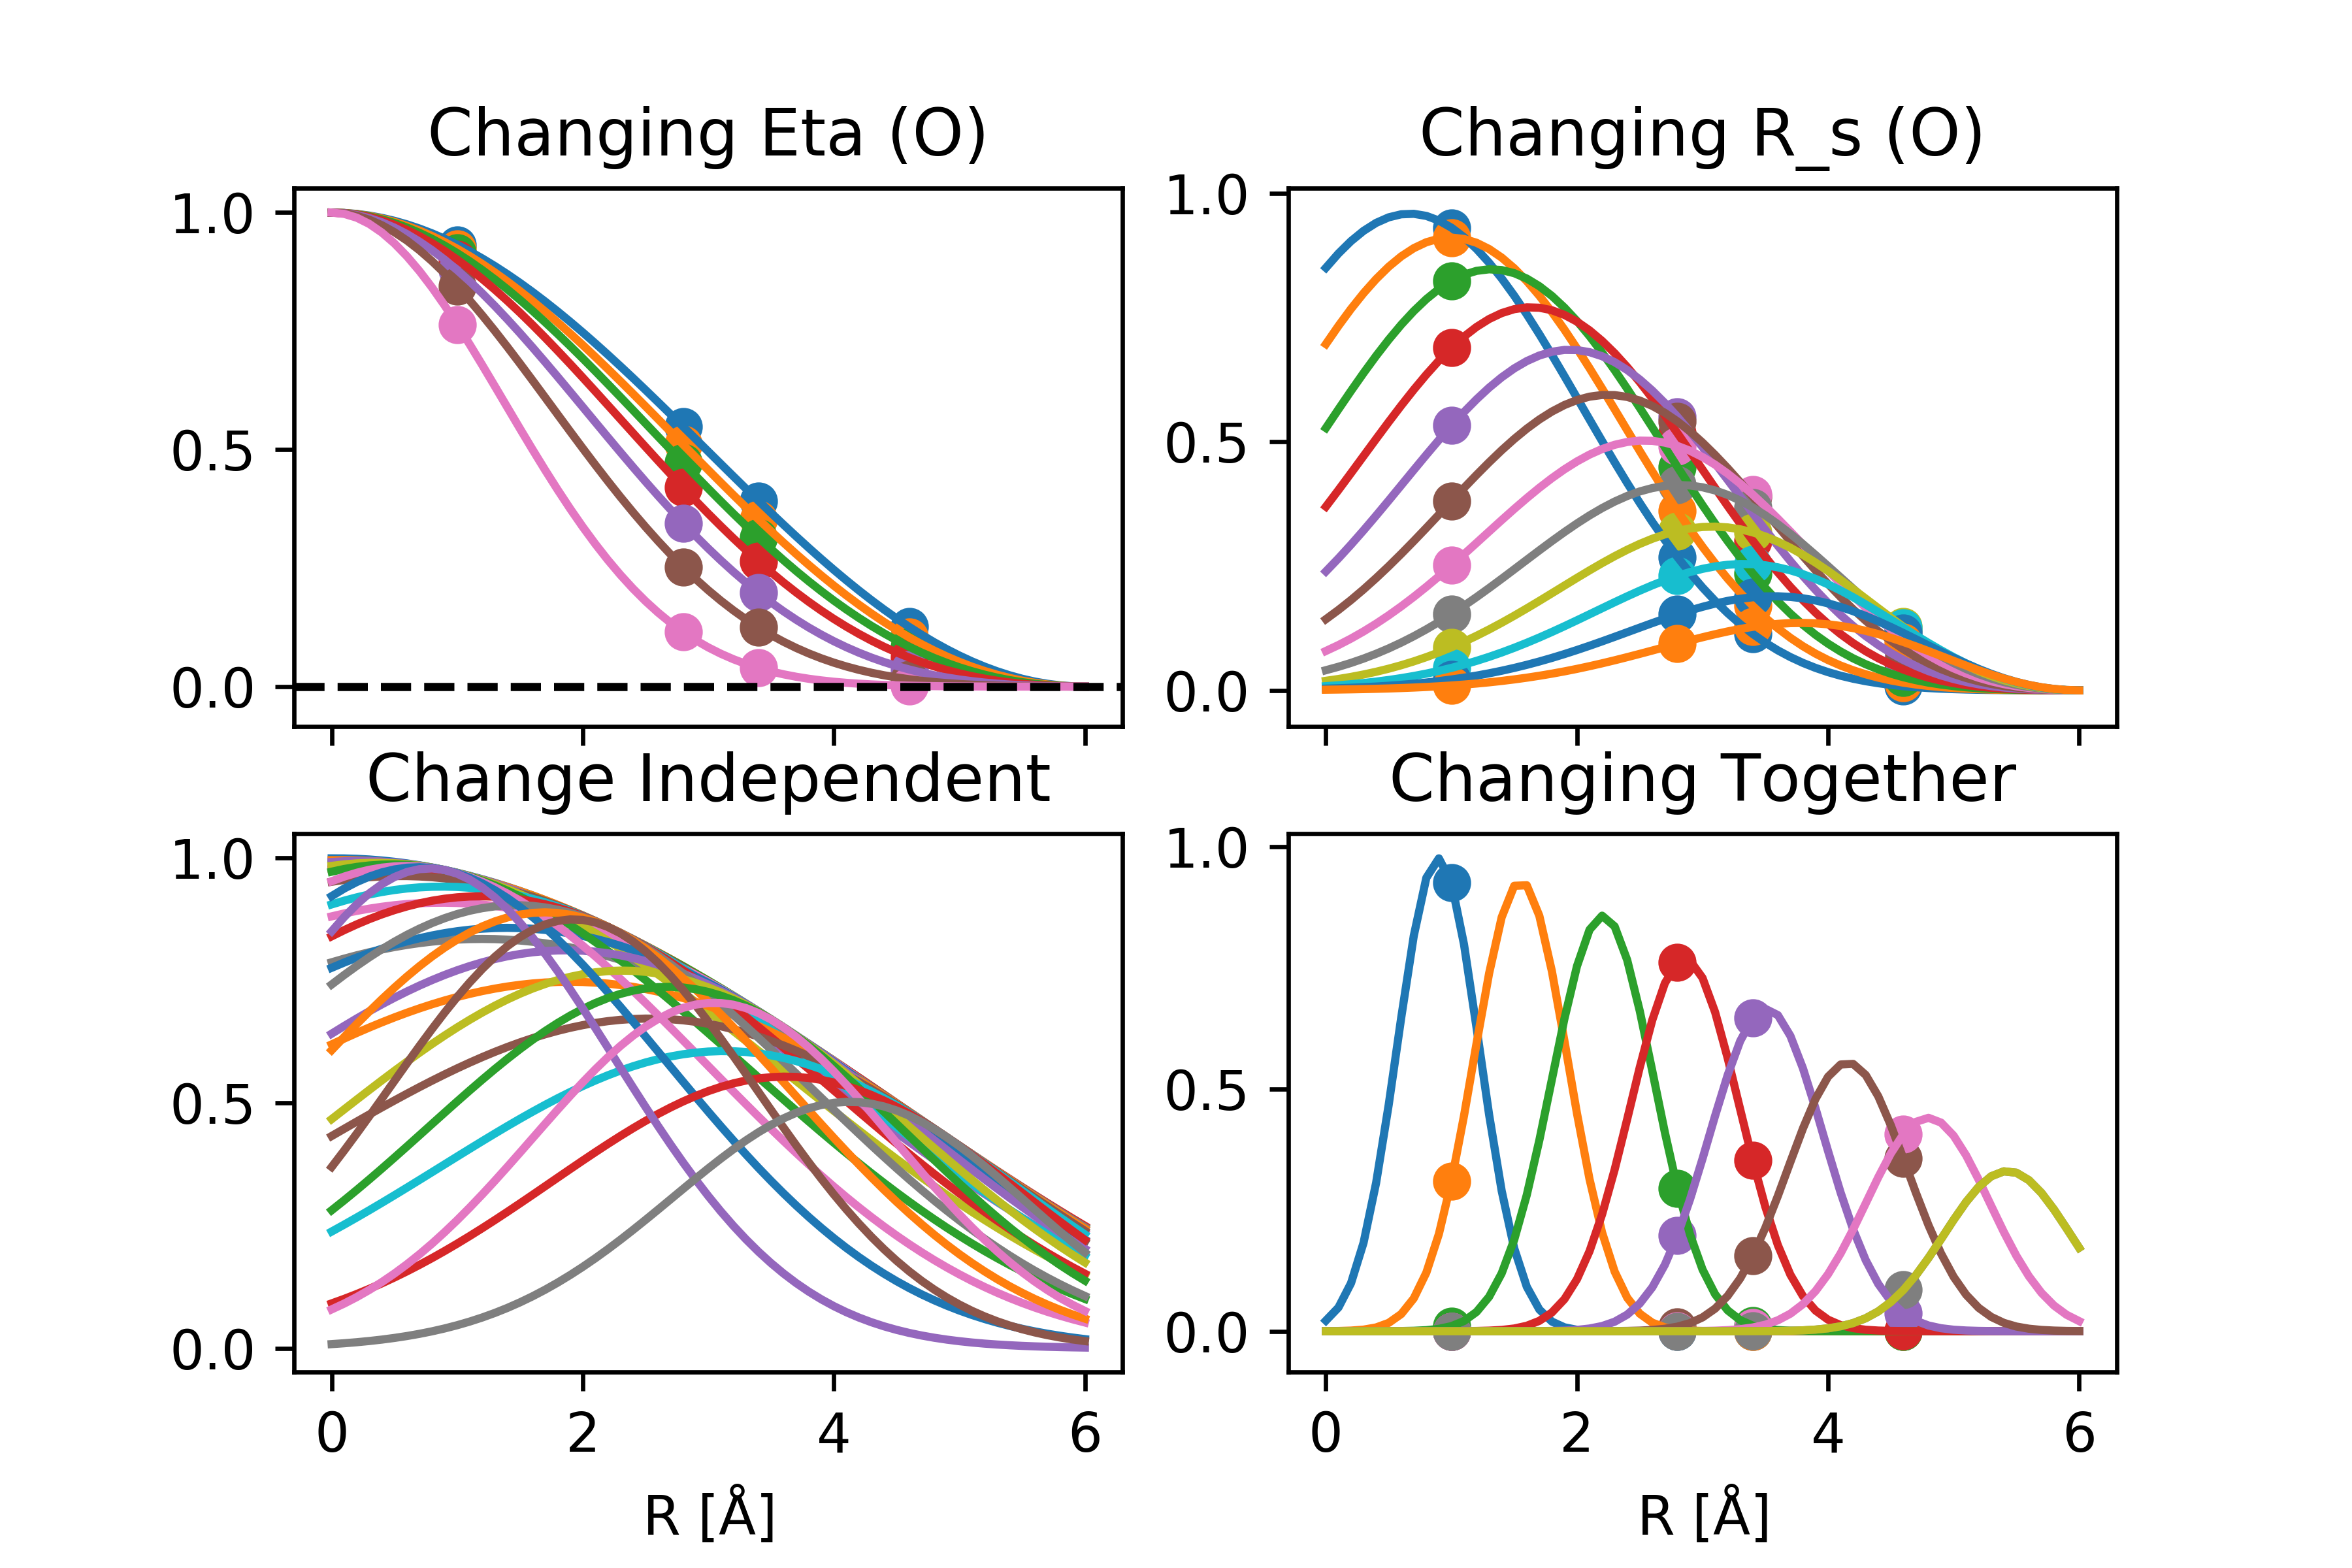
\includegraphics[width=\linewidth]{./img/rad_graphs.png}	\caption{Changes in radial basis function while adjusting parameters. The colored points represent the value of the symmetry function for an atom located at R $\mathrm{\AA}$ away from the given atom.}
	\label{fig:rad_funcs}
\end{figure}
\ref{fig:ang_funcs}
\begin{figure}
	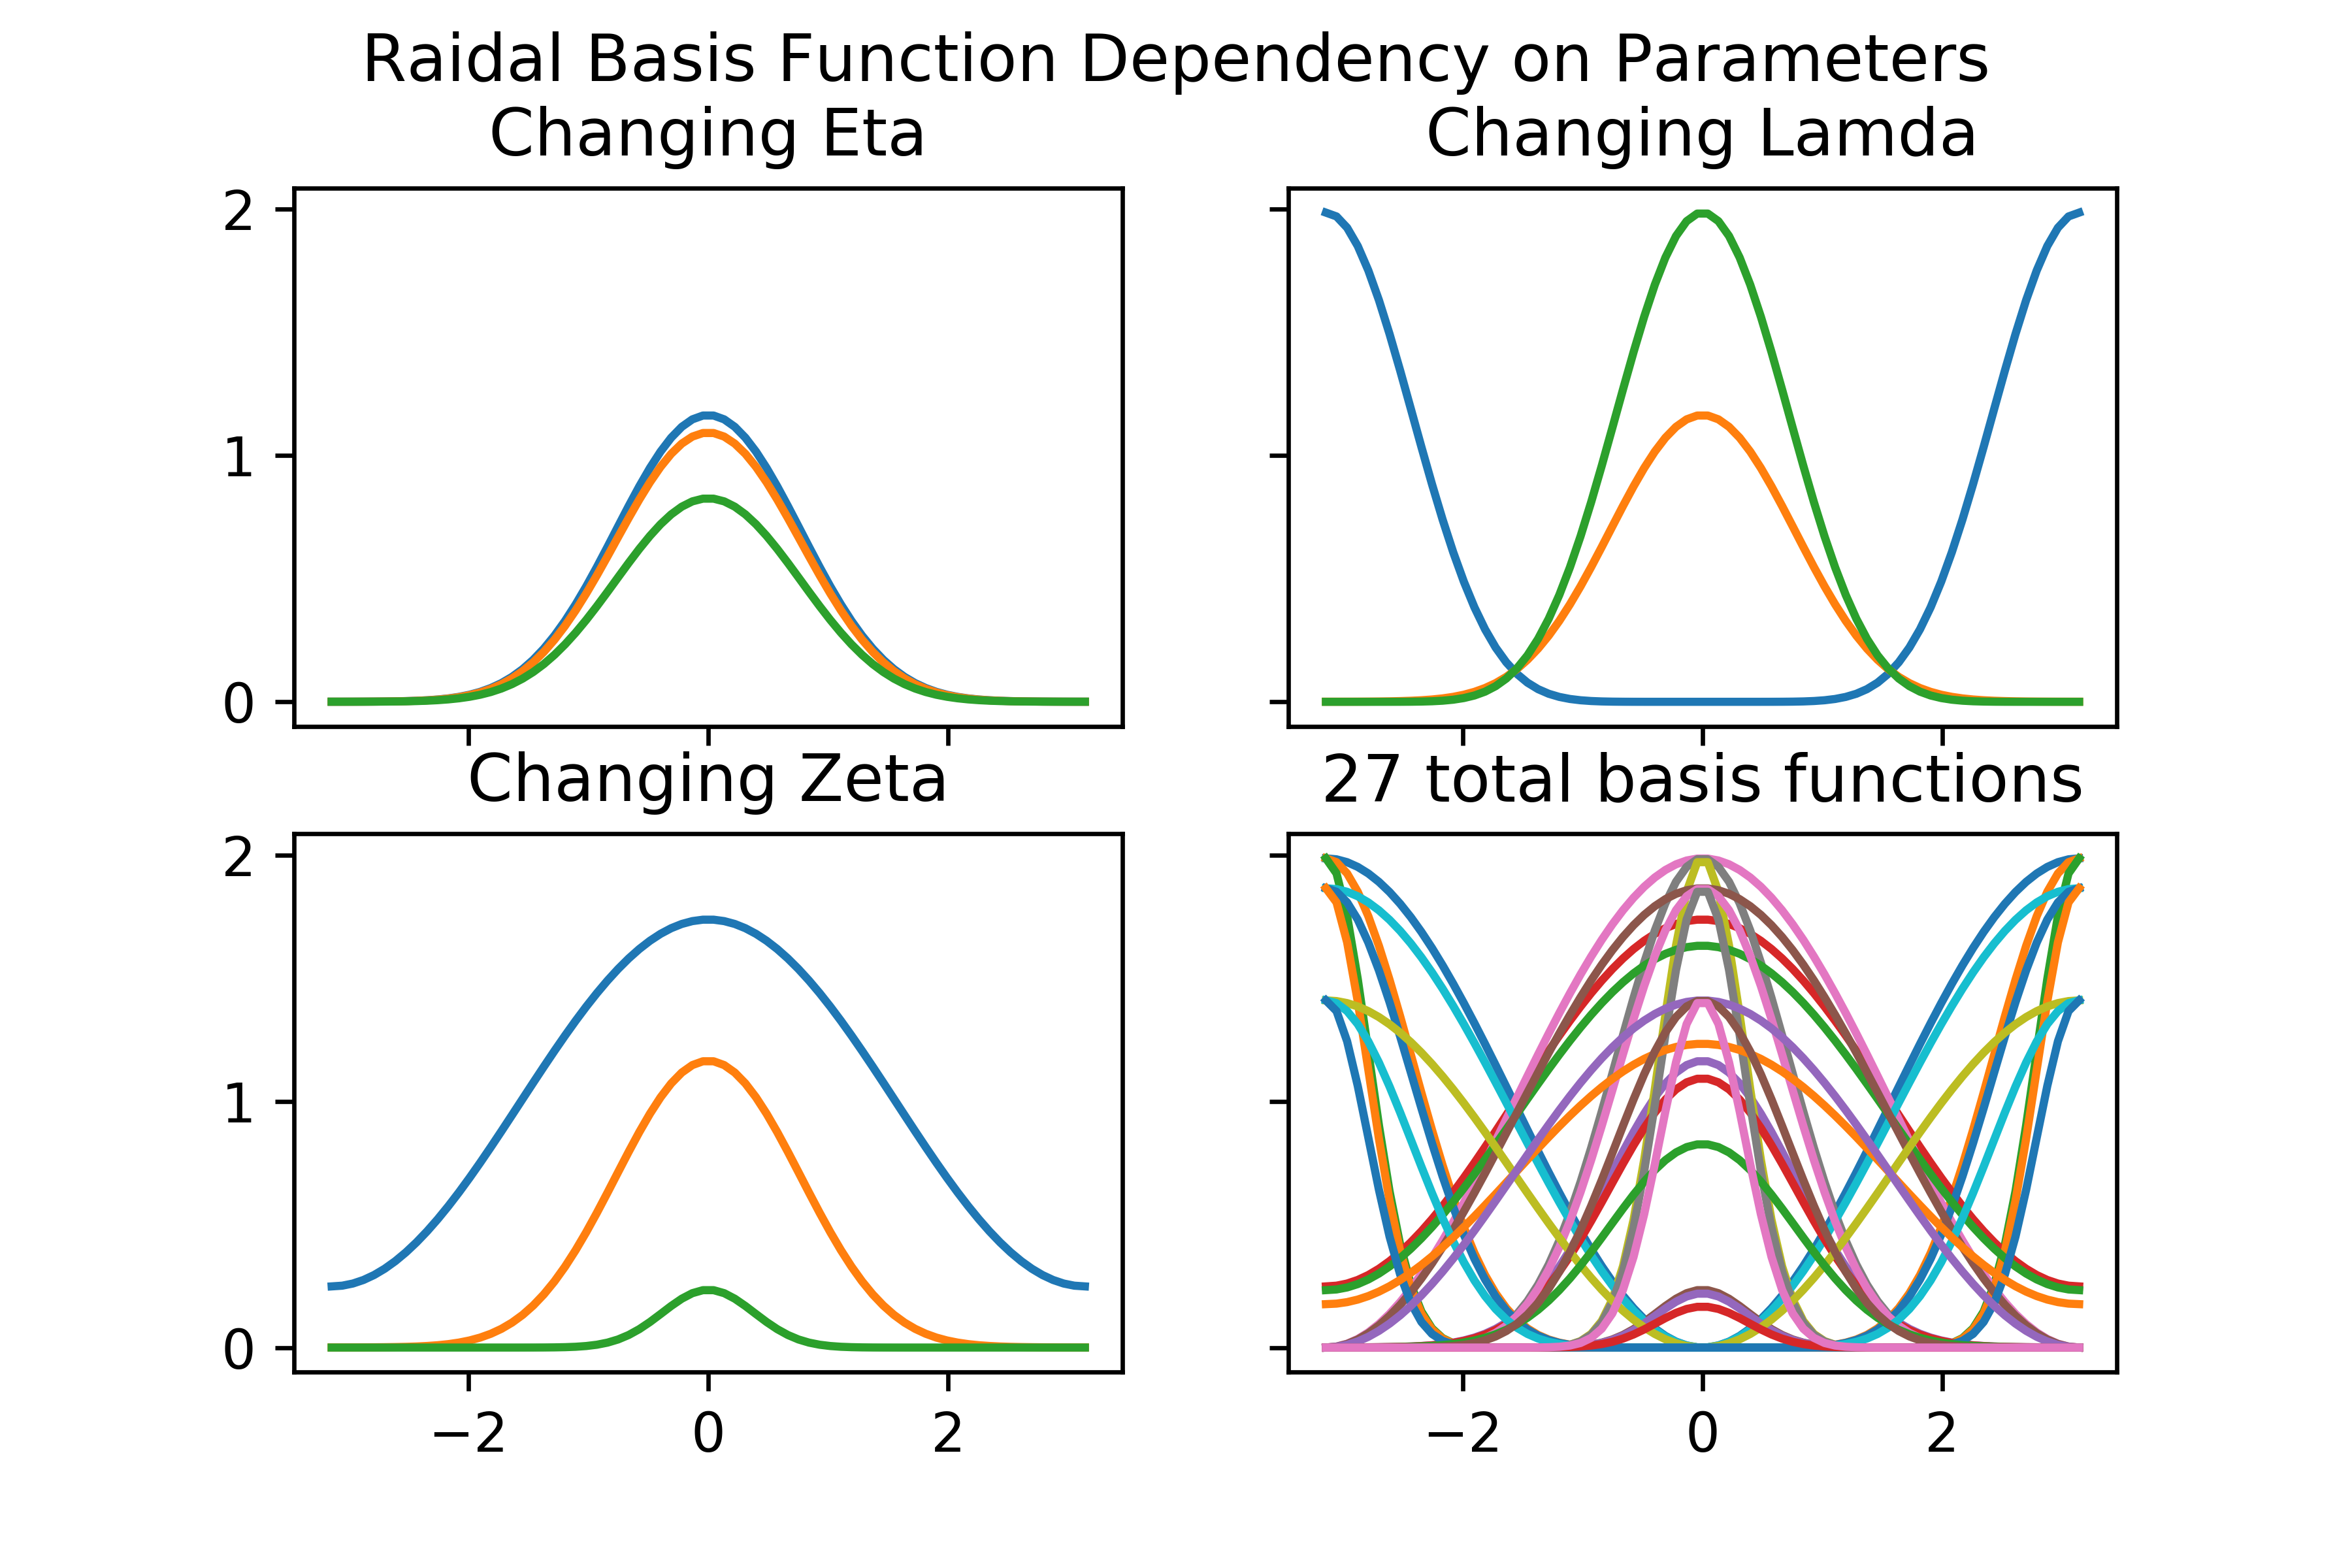
\includegraphics[width=\linewidth]{./img/ang_graphs.png}	\caption{Changes in angular basis function while adjusting parameters. The colored points represent the value of the symmetry function for an atom located at R $\mathrm{\AA}$ away from the given atom. This needs to be checked to ensure that equation 4 was used}
	\label{fig:ang_funcs}
\end{figure}
\newpage
\subsection{Symmetry Function Gradient}
The gradients of the symmetry function terms are presented here in order of increasing complexity.

The gradient of the distance $R_{ij}$ with respect to $i$ is the unit vector along the line between the two points:

\begin{equation}
\frac{\partial R_{ij}}{\mb{X}_{i}} = -\frac{\mathbf{X}_j-\mathbf{X}_i}{\lVert \mathbf{X}_j - \mathbf{X}_i \rVert} = -\frac{\mathbf{X}_j-\mathbf{X}_i}{R_{ij}}
\end{equation}

\begin{equation}
\frac{d R_{ij}}{d \mb{X}_{j}} = - \frac{\partial R_{ij}}{\partial\mb{X}_{i}}
\end{equation}

The gradient of the smoothing function with respect to the ${i}$-th cartesian coordinate:
\begin{equation}
\frac{\partial f_c (R_{ij}) } { \mb{X}_{i}} = -\frac{\pi}{2 
 \mathrm{R_s}}  \sin ( \frac{\pi R_{ij}}{\mathrm{R_s}}) \frac{\partial R_{ij}}{\mb{X}_{i}}
\end{equation}

The gradient of the $j$-th component of the $i$-th radial symmetry function:
\begin{equation}\label{eq:rad_derivative}
\frac{\partial G_{i,j}^2 } { \partial \mb{X}_i} = e^{-\eta ( R_{ij} - \mathrm{R_s} )^2} \left[ -2 \eta ( R_{ij} - \mathrm{R_s} )  f_c (R_{ij}) \frac{\partial R_{ij}}{\partial  \mb{X}_i} + \frac{\partial f_c ( R_{ij} )}{\partial \mb{X}_i} \right] 
\end{equation}

\subsubsection{Angular Symmetry Functions}

The angular symmetry function terms and gradients.

\begin{equation}
\frac{\partial } {\partial \mb{X}_i}
 e^{-\eta ` \left( R_{ij} + R_{ik} + R_{jk} \right)^2 } =
  -2 \eta` \left( R_{ij} + R_{ik} + R_{jk} \right) e^{-\eta` \left( R_{ij} + R_{ik} + R_{jk} \right)^2   } \left(
\frac{d R_{ij}}{\partial \mb{X}_i} + \frac{d R_{ik}}{\partial \mb{X}_i} \right)
\end{equation}

\begin{equation}
\frac{\partial } {\partial \mb{X}_i} ( 1 + \lambda \cos{\theta_{ijk}} )^\zeta  = \zeta ( 1 + \lambda \cos \theta_{ijk} ) ^ {\zeta - 1} \lambda\frac{\partial \cos \theta_{ijk} } {\partial \mb{X}_i}
\end{equation}

As $\cos \theta$ can be expressed as:

\begin{equation}
\cos \theta_{ijk} = \frac{\mb{R}_{ij} \cdot  \mb{R}_{ik}} { R_{ij}  R_{ik}}
\end{equation}

Here, the gradient with respect to $\mb{X}_j$ or $\mb{X}_k$ is:

\begin{equation}
\frac{\partial \cos \theta_{ijk} } {\partial \mb{X}_j} = -\frac{\cos{\theta}}{R_{ij}} \frac{\partial R_{ij}}{\partial \mb{X}_j} + \frac{\mb{R}_{ik}}{R_{ij} R_{ik}}
\end{equation}

The gradient with respect to $\mb{X}_i$ is:
%\begin{equation}
%\frac{\partial \cos \theta_{ijk} } {\partial \mb{X}_i} = -\frac{\mb{R}_{ij} \cdot \mathbf{R}_{ik}  }{ \left( R_{ij}  R_{ik} \right) ^ 2}  
%\left( R_{ik} \frac{\partial R_{ij} } {\partial \mb{X}_i} + R_{ij} \frac{\partial R_{ik} } {\partial \mb{X}_i} \right) + \frac{ 2\mb{X}_i - \mb{X}_j - \mb{X}_k} { R_{ij} R_{ik} }
%\end{equation}

\begin{equation}
\frac{\partial \cos \theta_{ijk} } {\partial \mb{X}_i} = -\frac{\cos{\theta}  }{  R_{ij}  R_{ik} }  
\left( R_{ik} \frac{\partial R_{ij} } {\partial \mb{X}_i} + R_{ij} \frac{\partial R_{ik} } {\partial \mb{X}_i} \right) + \frac{ 2\mb{X}_i - \mb{X}_j - \mb{X}_k} { R_{ij} R_{ik} }
\end{equation}

This is implemented as and equivalent to:
\begin{equation}
\frac{\partial \cos \theta_{ijk} } {\partial \mb{X}_i} = - \frac{\partial \cos \theta_{ijk} } {\partial \mb{X}_j} - \frac{\partial \cos \theta_{ijk} } {\partial \mb{X}_k}
\end{equation}

\section{Input File Format}

For the input file, list all of the keywords. Then list the BPSF data as per the section \ref{bpsfinput}.

\subsection{Keywords}

\begin{description}[style=unboxed, labelwidth=\linewidth, font=\sffamily\itshape\bfseries , listparindent=0pt, before =\sffamily]

\item[geom\_file (string)]
The file path to the HDF5 file which contains geometries for calculating BPSF functions.
This keyword has no effect in library mode, as the calling program will provide the geometries.

\item[max\_angle (int)]
The maximum number of angle types for BPSF calculations over all of the elements.

\item[max\_bond (int)]
The maximum number of bond types for BPSF calculations over all of the elements.

\item[max\_eta\_zeta\_lam (int)]
The maximum number of $\eta$, $\zeta$, and $\lambda$ triplets for all of the elements.
This is the maximum angular basis length.

\item[max\_rs\_eta (int)]
The maximum number of $R_s$ and $\eta$ pairs for over all of the elements.
This is the maximum radial basis length.

\item[num\_els (int)]
The number of elements for the BPSF calculations.

\item[parse\_cart\_grads (string)]
This keyword signals to the program to parse the cartesian gradients from the input file specified by the \texttt{geom\_file} keyword.
Please provide the HDF5 key for the cartesian geometries in the file.
The geometries must be stored in an array with dimensions [number of geometries, number of atoms, 3].

\item[rc (float)]
This is the $R_c$ cutoff parameter for the BPSF symmetry functions described in Equation \ref{eq:rad}.

\item[timing\_interval (int)]
This is the nuber of steps between timing ouptuts when calculating BPSFs from an input file.

\item[verbose (str)]
Print voluminous information. You must put any string after the keyword as all keywords must have 2 words. 

\end{description}
\subsection{BPSF Input}\label{bpsfinput}

\section{Interface Module}
The interface module consists of wrapper code for C++ libraries RapdiJSON and Libcurl.
A C API wraps the TensorFlow Serving object class in the C++ code. 
There is a FORTRAN interface connected to the C API which provides FORTRAN bindings for each of the functions in the C API.
Through the C and FORTRAN APIs, the functionality of this code should be available to programs written in most languages.
The FORTRAN API can be found in the source code \texttt{tfserving\_utils\_mod.f03} and the C API in \texttt{tfserving\_utils\_capi.cpp} .

\subsection{Example of Interface via Fortran}
Create an variable of the TFServing Object.

\begin{lstlisting}[language=Fortran]
use iso_c_env
use libserving
type(tfserving) :: tfs
integer(c_int) :: port
integer(kind=4) :: port2 ! Can use this if you don't want to use C vars
character(len=:), allocatable :: model_name
port = 8500
model_name = "bpsf"
! Initialize the fortran interface with this tfs object
tfs\%initialize(port, model_name)
! Call a function that wraps the BPSF calculation
tfs\%wrapBPSF(coords)
! Cleanup. Optional for ifort and GCC > 7.0
tfs\%delete()
\end{lstlisting}

\subsection{Interface Subroutines}
The following subro:qutines can be called by the Fortran interface:

\section{Utility Scripts}
\subsection{compare basis functions}
Compares the basis functions between two HDF5 files.
This is used extensively for debugging to ensure that the HDF5 files are the same as a given standard.

\subsection{create input file}
This subroutine parses an input file written in a more lax standard and ouptuts the BPSF section in the exact format that the FORTRAN program wants it.
Therefore, this can be used in lieu of manually following the confusing specifications.

\subsection{indicator tools}
This contains helper functions

\subsection{scan hdf5}
This script performs a similar function to the command h5ls: it goes through an HDF5 file and prints out the keys and shapes for each dataset.

\subsection{tf sym funcs}
This very slow program is verified to produce the exact radial and angular basis functions for sets of atoms.
The slowness of this program compelled the authors to write this code.

\subsection{xyz nn analysis}
Compresses a folder of \texttt{.xyz} files into an HDF5 file.


\section{Tests}
\subsection{Test 1 - Comparing answers with reference}

\subsection{Test 2 - Calculation of the radial gradient}
In this test, a simple system was constructed to check the numerical accuracy of the gradient calculations. The O-H molecule was constructed, with the O-H bond measuring 1.0 $\mathrm{\AA}$ and lying along the $x$-axis. The $y$ and $z$ coordinates were all set to 0. Thus, the derivative of the radial symmetry functions should only be non-zero in the $x$ direction, and the result can be easily checked. Additionally, the gradient should be symmetrical between the O and the H atoms.The answers are presented here. The ith atom is the O with coordinates of (-1, 0, 0| and the jth atom is the H with coordinates (1, 0, 0).


$\eta = 19.53125$

$\mathrm{R_s} = 0.8$

$\frac{\partial R_{ij}}{\partial x} = 1$

$\frac{\partial f_c (R_{ij}) } { \partial x} = - \frac{\pi}{2 * 0.8} sin \left( \frac {\pi}{0.8} \right) * 1 $

From equation \eqref{eq:rad_derivative}, the final answer can be calculated:

$\frac{\partial G^2_{ij}}{\partial x} = -3.475089$

\subsection{Test 3 - Calculation of the Angular Gradient}
Here, the angular gradient is calculated for a couple geometries.
The "correct answers" for the output of the file should be here.

\begin{center}
\begin{tabular}{ |c|c| }
Variable     & Value \\
$X_i$        &  0.0 0.0 0.0 \\
$X_j$        &  0.0 1.0 0.0 \\
$X_k$        &  1.0 0.0 0.0 \\
$\eta$       & 0.001 \\
$\zeta$      & 1 \\
$\lambda$    & -1 \\
$\cos$       & 0 \\
'gauss term' & 9.884108 \\
dgauss di    & 6.74929E-3 \\
dgauss dj    & 6.74929E-3 \\
dgauss dk    & 0 \\
cos term     & 1.0 \\
fc product   & 0.855794 \\
i final gradient & 0.917726 \\
j final gradient & 0.917726 \\
k final gradient & 0

\end{tabular}
\end{center}


\subsection{Test 4 - Parallel Compare}
The output of this file should be the same as the output of test 3.

\subsection{Test 5 - Call as a library}
This example shows code that uses FORT-BPSF as a library.

\subsection{Test 6 - Call with JSON Interface}
\subsection{Test 7 - }
\subsection{Test 8 - }
\subsection{Test 9 - }
\subsection{Test 10 - }
\subsection{Test 11 - }
\subsection{Test 12 - Example of parse\_cart\_grad keyword}
Here, the cartesian gradients are parsed from a benchmarking file with 1,000 geometries and energies, and added to the resulting \texttt{output.h5} file.

\section{Developer's Guide}
This section contains notes as to the inner workings of the program.
It is only likely useful if someone needs to modify the program.

\subsection{Coordinate, Atomic Number, and Num Atoms H5 Input}
The HDF5 dataspaces for these files as well as the dimensions of these datasets are found in the \texttt{FI init from ifi} subroutine.
The arrays are filled in the \texttt{FI get data} subroutine.
The input file and data spaces are then closed in the \texttt{FI clean inputs} subroutine.

\subsection{Atom Based Cartesian Gradients}
This section behaves differently than the above data as the values parsed here are not needed for BPSF calculations.
I thought it would be better to encapsulate all of these calls so that this can be later moved to after the BPSF calculation, or these could be written and removed from memory to save memory.
The hdf5 dataspace is still opened in the subroutine \texttt{FI\_init\_from\_ifi}, but the rest of the parsing and closing of the data is done in the subroutine \texttt{FI\_get\_data}.


\end{document}